%% This is an example first chapter.  You should put chapter/appendix that you
%% write into a separate file, and add a line \include{yourfilename} to
%% main.tex, where `yourfilename.tex' is the name of the chapter/appendix file.
%% You can process specific files by typing their names in at the 
%% \files=
%% prompt when you run the file main.tex through LaTeX.
\chapter{Overview of Visual-inertial Odometry}
\label{chap:Overview}

In this chapter, we will overview visual-inertial odometry system. In section
\ref{sec:notations}, we will introduce world representation(\eg, world frame,
camera frame and IMU frame) together with basic notations in our odometry system. 
Then in section \ref{sec:FVK}, 
we will discuss two important scheme, filter method and keyframe Bundle 
Adjustment(keyframe BA) in SLAM algorithm, and explain why we finally choose
keyframe-based method.

\section{World Representations and Notations}
\label{sec:notations}

Visual-inertial odometry~\cite{li2011consistency}, literally, is an odometry
system, which received
environment information by visual (camera) and inertial (IMU) sensor.
VIO is similar with well-known visual odometry (VO) problem \cite{nister2004visual},
with an additional IMU sensor, it tries to estimate agent's pose as agent keep moving
in the environment. One big difference between VIO and SLAM algorithm is that VIO
does not or only build a simple map, whereas SLAM normally maintains and continuously
updating a map.

To setup a VIO system, we need to first define the ways to represent the world. Globally,
we have a world frame $\W$; World frame $\W$ is set to a right-handed Cartesian 
coordinate system that every objects has an absolute pose (translation and rotation) in
it. Then we have local frame for each sensor, \ie, IMU frame $\I$ and camera frame $\C$;
Every time camera and IMU sensor obtain observations within their own local frame, we
need to integrate those data and estimate the pose of those sensors in world frame $\W$.
Figure \ref{fig:fig2-1} shows the overall world representations. 

\begin{figure}[t]
    \centering
    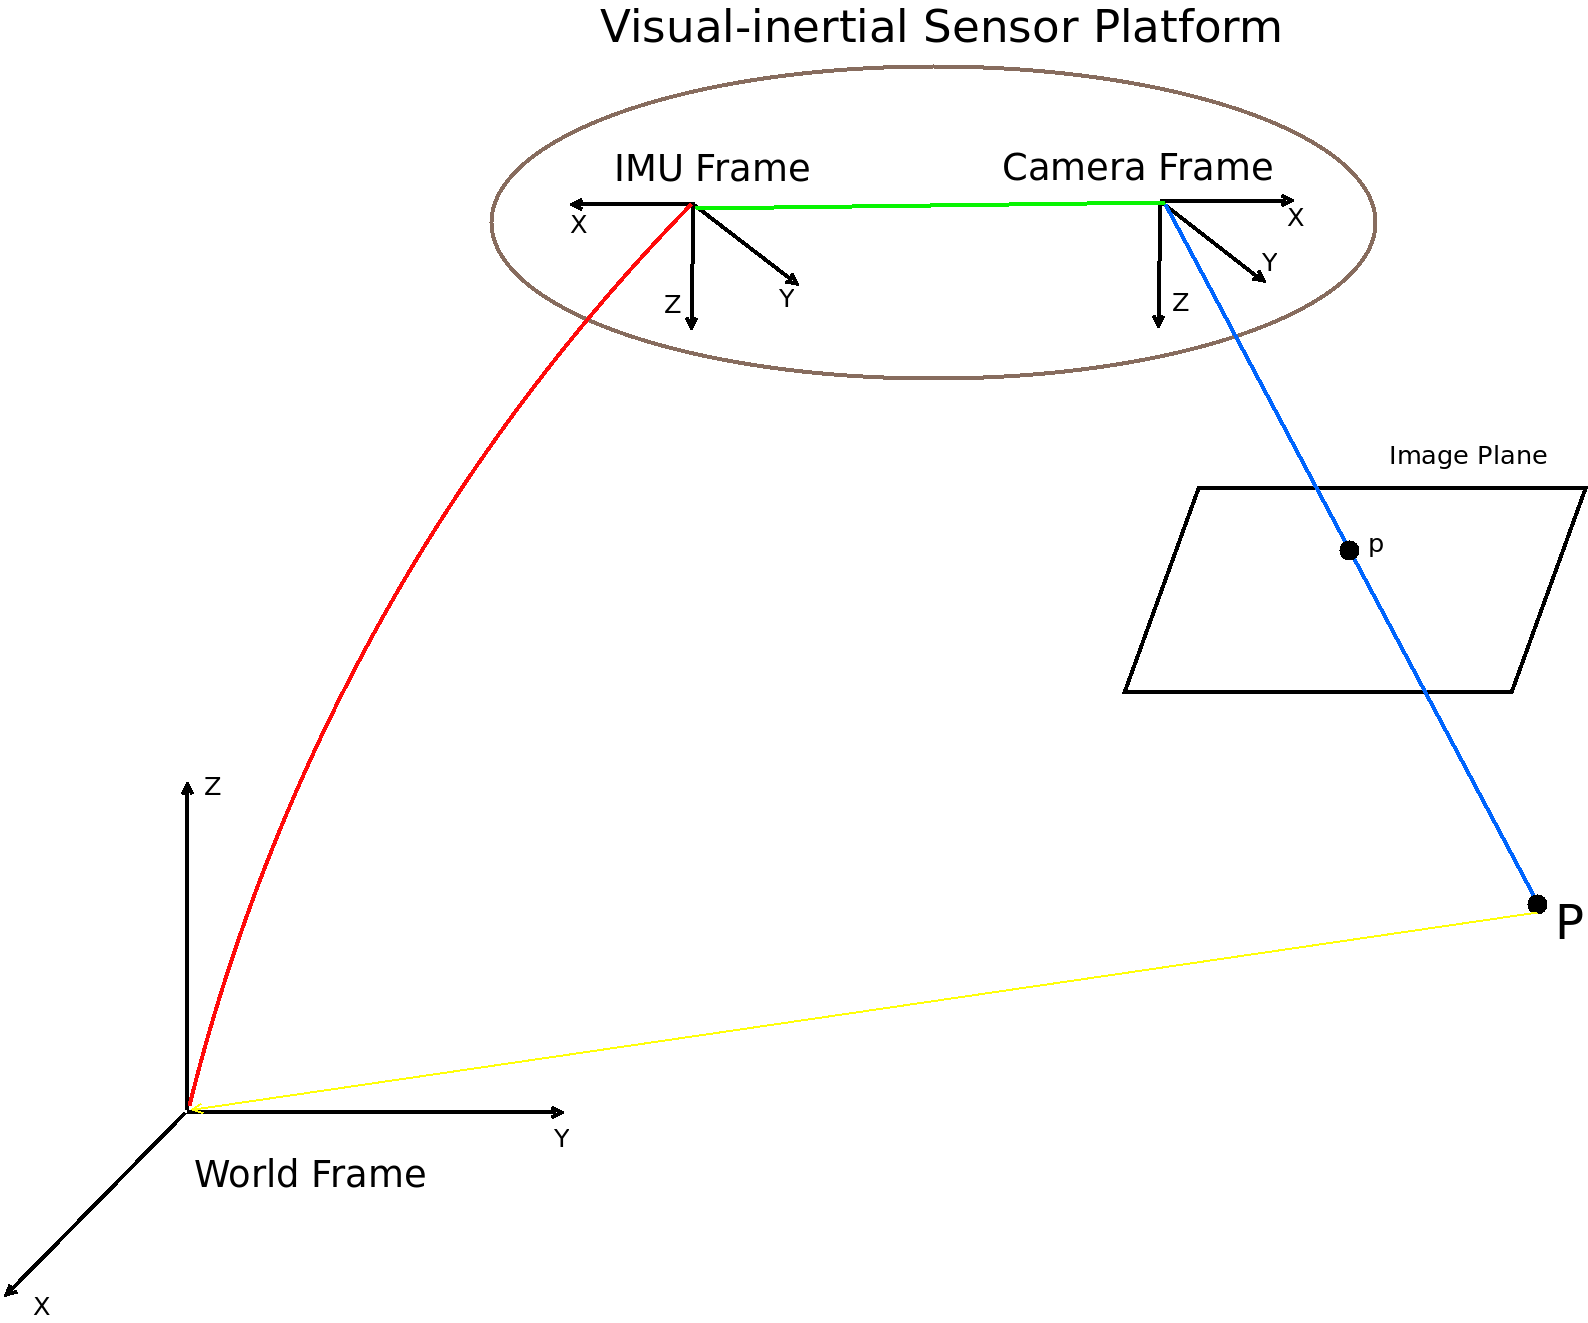
\includegraphics[width=0.5\textwidth]{CONTENT/Figure/Figure2-1_World.png}
    \caption{This figure shows the connection among world frame $\W$, IMU frame $\I$
    and camera frame $\C$. Green line shows the transformation between camera and
    IMU, which can be pre-calibrated. Red line is the pose of IMU in world frame.
    Camera frame observes point p of object P in image plane, andconnects a object P by
    blue line, and the coordinate of object P
    in world frame is presented as yellow line.}
    \label{fig:fig2-1}
\end{figure}

In this master thesis, we denote measurement $M$ in particular frame $\F$ as $M_{\F}$. 
To further simplify, any parameter that is \textbf{not} in world frame shall 
be denoted particularly. For example, the translation $P$ in camera frame will 
be denoted as $P_{\C}$, and the translation $P$ in world frame will 
be denoted as $P$. 


\section{Filter Versus Keyframe}
\label{sec:FVK}
   